% !TeX root = ../Thesis.tex

%************************************************
\chapter{Design}\label{ch:design}
%************************************************
\glsresetall % Resets all acronyms to not used

In this chapter, we will discuss the important design decisions for our implementation of text-based steganography on Android. First, we will investigate what options currently exist to run \glspl{LLM} locally. Then, we will show how to select a suitable \gls{LLM} for our use case.

We will focus on the technologies that are unique to our implementation, therefore the full tech stack shall only be mentioned here briefly:
\begin{itemize}
	\item The app is written in Kotlin~\cite{kotlinKotlinProgrammingLanguage}, with Jetpack Compose as a \gls{UI} framework.
	\item Besides the Android \gls{SDK}, we use the \gls{NDK} to integrate some C++ code into our app.
	\item The \gls{LLM} is run using the llama.cpp library~\cite{gerganovGgerganovLlamacpp2024}.
	\item Our \gls{IDE} of choice is Android Studio, which comes with Gradle~\cite{gradleGradleBuildTool2025} as a build system (includes CMake~\cite{cmakeCMakeUpgradeYour} via the \gls{NDK}).
\end{itemize}

Furthermore, the following dependencies were added to the default Android Studio project (in chronological order of commits):
\begin{itemize}
	\item The Androidx Navigation Compose library for navigation between screens.
	\item The Androidx Material Icons Extended library for some icons.
	\item The Androidx DataStore Preferences library to store app settings.
	\item The Androidx Room library to access a local SQLite database (requires \gls{KSP} plugin~\cite{googleGoogleKsp2025} for annotations).
	\item The Kotlinx Serialization library~\cite{kotlinKotlinKotlinxserialization2025} for serialization.
\end{itemize}

By preferring native Android and Kotlin libraries, we introduce as little third party dependencies as possible. This aligns with the requirements detailed in \cref{sec:makingAVirtueOutOfNecessity}.

\section{How to run large language models on Android}
\label{sec:howToRunLLMsOnAndroid}
When approaching the topic of this thesis, the first major task was to research ways to run a \gls{LLM} locally on an Android smartphone. The Android platform restricts our choice of runtime environments to those that support the \gls{JVM}~\cite{ruggiaDarkSideNative2025}. Relevant programming languages therefore are Java, and by extension, Kotlin. Other programming languages that compile to Java Byte Code exist (e.g. Scala), but are not well-supported on Android~\cite{ruggiaDarkSideNative2025}. Furthermore, we have the option of including C++ code into our Android app by using the Android \gls{NDK}. Communication between Java/Kotlin and C++ code is facilitated via the \gls{JNI}~\cite{ruggiaDarkSideNative2025} (see \cref{ch:implementation} for details).

\subsection{PyTorch}
\label{sec:pyTorch}
The core paper this thesis is based on is Stegasuras~\cite{zieglerNeuralLinguisticSteganography2019}, which is written in Python. It uses the PyTorch and HuggingFace Transformers libraries to run the \gls{LLM}~\cite{zieglerStegasuras2025,anselPyTorch2Faster2024,wolfTransformersStateoftheArtNatural2020}. Originally being developed by Facebook (now Meta) since 2016, PyTorch is part of the Linux Foundation since 2022~\cite{chintalaPyTorchStrengthensIts2022}. It also comes with its own tensor library called ATen~\cite{devitoZdevitoATen2025}. Therefore, finding a way to run PyTorch on Android was the obvious first approach. Unfortunately, Python support on Android is not officially endorsed by Google. Some language bindings to Kotlin or Java exist for PyTorch, but none of them are actively maintained. While some libraries for building cross-platform Python applications exist~\cite{kivyKivyKivy2025,beewareBeewareToga2025,chaquoChaquoChaquopy2025}, they share a common concern. As Python integration requires another abstraction layer, this could introduce significant performance drawbacks, conflicting with our requirement of acceptable performance on entry-level smartphones. Ultimately, no option was attractive enough to commit to working with it.

Furthermore, the industry is centered around Kotlin as the language officially endorsed by Google~\cite{ruggiaDarkSideNative2025}. Java as its predecessor is being phased out, but its libraries remain interoperable with Kotlin. C++ is not as preferred, since its manual memory management makes it prone to security vulnerabilities~\cite{ruggiaDarkSideNative2025}. The PyTorch ecosystem offers multiple distributions that might help us here~\cite{pytorchPyTorch}:
\begin{itemize}
	\item PyTorch, the original Python library~\cite{anselPyTorch2Faster2024}.
	\item PyTorch Mobile, for Android and iOS~\cite{pytorchPytorchAndroiddemoapp2025}.
	\item ExecuTorch, for Android and iOS~\cite{pytorchPytorchExecutorch2025}.
	\item libtorch, the Java and C++ distributions of PyTorch~\cite{pytorchStartLocally,pytorchPyTorchAPIPyTorch}.
\end{itemize}

Upon closer inspection, none of them seemed production-ready for Android. PyTorch Mobile is no longer maintained~\cite{pytorchPytorchAndroiddemoapp2025}, while ExecuTorch was still in its beta phase~\cite{pytorchPytorchExecutorch2025}. Information about libtorch was conflicting, as in some places of the documentation it was claimed to be stable, while others marked it as unstable~\cite{pytorchStartLocally,pytorchPyTorchAPIPyTorch}. While libtorch might work otherwise, it would require us translating all of the Stegasuras code to C++. As explained earlier, this is not to be preferred for maintainability. Furthermore, there was a lack of both open source projects using PyTorch on Android and \glspl{LLM} readily available on platforms like HuggingFace~\cite{huggingfaceModelsHuggingFace2025}. While a lot of base models are available in PyTorch format, their quantizations are not (see \cref{sec:llamaCpp} and \cref{sec:howToSelectASuitableLLM} for details). Ultimately, these approaches were ruled out because the expected compromises could not be justified.

\subsection{TensorFlow}
\label{sec:tensorFlow}
TensorFlow, developed by Google since 2015, is a popular competitor to PyTorch~\cite{abadiTensorFlowLargescaleMachine2015}. It is often said that PyTorch is more popular amongst researchers, while TensorFlow is more popular amongst businesses. It too comes in multiple distributions:
\begin{itemize}
	\item TensorFlow, the original Python library~\cite{abadiTensorFlowLargescaleMachine2015}.
	\item LiteRT (formerly TFLite), for Android and iOS~\cite{googleaiedgeteamTensorFlowLiteNow2024,googleGoogleaiedgeLiteRT2025}.
\end{itemize}

Language support is on par with PyTorch, as Python, C++ and Java are listed in the documentation~\cite{tensorflowTensorFlow}. Unfortunately, only the Python library was stated to be stable. The Java and C++ distributions were either marked unstable or had conflicting information~\cite{abadiTensorFlowLargescaleMachine2015,tensorflowAPIDocumentationTensorFlow}. While this implies some of the same trade-offs we had with PyTorch, the TensorFlow ecosystem is a lot less fragmented. Even hardware acceleration on mobile devices is prominently mentioned in the TensorFlow documentation~\cite{tensorflowTensorFlow}. This made TensorFlow seem like a more promising solution than PyTorch, but using it would mean translating all the Stegasuras code~\cite{zieglerHarvardnlpNeuralSteganography2025} to both another language and framework. Unfortunately, TensorFlow suffers from the same lack of community projects using it for \gls{LLM} inference on Android as PyTorch does. Furthermore, just like with PyTorch, a lot of the base models on HuggingFace~\cite{huggingfaceModelsHuggingFace2025} were available in TensorFlow format, but not their quantizations (see \cref{sec:llamaCpp} and \cref{sec:howToSelectASuitableLLM} again for details). For these reasons, TensorFlow was not chosen either.

\subsection{llama.cpp}
\label{sec:llamaCpp}
As investigating the popular PyTorch and TensorFlow ecosystems didn't yield any obvious example projects from the open source community, we changed our research approach. Instead of looking for frameworks and then trying to find examples, we now looked for examples to then find out what frameworks they used. We searched the Google Play Store and GitHub for Android apps that offered a chat functionality with local \glspl{LLM}. This approach was more successful, as we found three apps that use the same framework: llama.cpp~\cite{panchalShubham0204SmolChatAndroid2025,vali-98Vali98ChatterUI2025,ghorbaniAghorbaniPocketpalai2025}. While these apps are projects by hobbyists, they allowed us to judge llama.cpp by seeing it in action.

We installed the apps onto a Moto One Vision, the Android phone used during most of the development (see \cref{sec:howToSelectASuitableLLM} for details). By today's standards, a Moto One Vision with its 4 GiB of memory is an entry-level phone. Performance was deemed acceptable if the \gls{LLM} was able to generate a response with at least 1 token/second throughout a small conversation of ten messages. Of course, we may be more ambitious with our own implementation. But since these were the first implementations we can test on Android, we gave them a bit of leeway.

All three apps allowed the user to run any \gls{LLM} from a \lstinline|.gguf| file~\cite{panchalShubham0204SmolChatAndroid2025,vali-98Vali98ChatterUI2025,ghorbaniAghorbaniPocketpalai2025}. We tested them with a 4 bit quantization of Llama 3.2 1B (see \cref{sec:howToSelectASuitableLLM} for details). All apps performed more than acceptably, generating responses with around 5 tokens/second. These results gave us confidence that we can fulfill our performance requirement with llama.cpp.

With this insight, llama.cpp was researched further. It became apparent that llama.cpp offered various benefits over both PyTorch and TensorFlow. Developed by Georgi Gerganov since 2023, it does not have any third party dependencies~\cite{gerganovGgerganovLlamacpp2024}. A vast selection of \glspl{LLM} on HuggingFace is quantized from their base model using llama.cpp~\cite{huggingfaceModelsHuggingFace2025}. Quantizations are stored as \lstinline|.gguf| files, which are self-contained, i.e. the \gls{LLM} is reduced to a single file~\cite{huggingfaceGGUF}. Both PyTorch and TensorFlow require the \gls{LLM} to be stored as a number of files. This ensures us that we can fulfill another requirement, namely making the \gls{LLM} swappable. Furthermore, llama.cpp is both very popular by itself (e.g. by GitHub stars) and as a library to be included in other software (e.g. in LM Studio, Ollama)~\cite{gerganovGgerganovLlamacpp2024}. Furthermore, its GitHub repository contains a number of examples for basic usage and a demo Android app that we can use as orientation~\cite{gerganovGgerganovLlamacpp2024}. Lastly, it comes with its own tensor library, ggml~\cite{gerganovGgerganovGgml2024}. This makes a complete software suite for \glspl{LLM}: llama.cpp as the runtime, ggml for tensor operations, \lstinline|.gguf| as file format.

Of course, llama.cpp has some downsides too. As it is a C++ library, it will make our implementation harder to maintain. It is still very young for a project of this complexity, so it is expected to not be stable for a while. But seeing it work in practice was good enough of an argument to commit to it. Experience throughout the course of this thesis will show that llama.cpp was a good choice. It offers significantly better abstractions than PyTorch, hiding tensor operations largely away (see ~\cref{ch:implementation} for details). Our implementation turned out to be easier to understand and work with than the original PyTorch implementation of Stegasuras~\cite{zieglerHarvardnlpNeuralSteganography2025}. Furthermore, performance of our implementation was good out of the box, with more optimization options to investigate (e.g. setting compiler flags for specific hardware architectures).

\subsection{Other options}
\label{sec:otherOptions}
Besides the three major frameworks discussed above, we also investigated many others. To eventually consider them in future projects, we present a selection of the most noteworthy ones here:
\begin{itemize}
	\item Jax, developed by Google, is being marketed as a possible successor to TensorFlow~\cite{jaxJaxmlJax2025}. As it is still a research project, it is not an official Google product yet. The main problem was again the availability of \glspl{LLM} in the required format.
	\item ONNX Runtime, developed by Microsoft, promises to be a unified runtime for \glspl{LLM} across formats, platforms and programming languages~\cite{onnxruntimedevelopersONNXRuntime2018,onnxruntimeONNXRuntimeHome}. While this means it could support quantized \glspl{LLM} in the \lstinline|.gguf| file format, availability of example projects was an issue again.
	\item llamafile, developed by Mozilla, promises to run \glspl{LLM} from a single file~\cite{mozillaMozillaOchoLlamafile2025,hoodIntroducingLlamafileMozilla2023}. As it is built on top of llama.cpp, which already does this, there is no obvious benefit for us.
\end{itemize}

We considered a number of projects more specific to Java/Kotlin as well, but dropped them mostly due to lack of popularity and active maintenance.

\section{How to select a suitable large language model}
\label{sec:howToSelectASuitableLLM}
With llama.cpp selected as the runtime environment, we have a wide variety of compatible \glspl{LLM} readily available in the \lstinline|.gguf| file format~\cite{huggingfaceModelsHuggingFace2025}. Now we need to investigate which \glspl{LLM} are suitable for our use case.

As we require our implementation to run on entry-level smartphones, hardware is the most limiting factor. More specifically, the amount of usable memory needs to be large enough to hold the \gls{LLM}, plus some overhead for the app process itself. \cref{tab:smartphones} gives an overview of the smartphones we used for testing. The baseline device is a Moto One Vision. Released to market in 2019, it can be considered entry-level by today's standards. According to the developer settings, around 1.5 GiB out of its 4 GiB of memory are available to applications, with the rest being occupied by the Android operating system. This suggests that we should be able to run \glspl{LLM} with a file size of around 1 GiB on it. Since our Moto One Vision is a typical smartphone with stock hardware and software, we expect this limitation to be similar on current entry-level devices.

\begin{table}
	\centering
	\begin{tabular}{@{} lr @{}} % @{} removes white spaces
		\toprule
		\tableheadline{Device} & \tableheadline{Memory} \\
		\midrule
		Moto One Vision          &  4 GiB \\
		Moto E13                 &  8 GiB \\
		Samsung Galaxy S24 Ultra & 12 GiB \\
		\bottomrule
	\end{tabular}
	% Use alternative short title for table of contents
	\caption[Smartphones used in evaluation]{Smartphones used for performance evaluation.}
	\label{tab:smartphones}
\end{table}

Initially, this was good enough to browse HuggingFace~\cite{huggingfaceModelsHuggingFace2025} and find some \gls{LLM} that would run on our hardware. But to make an educated decision, we need to understand which specifications of a \gls{LLM} determine its resource usage and output quality. The most detailed information about a specific \gls{LLM} can be found in the model card, which effectively is the \lstinline|README.md| of its repository~\cite{mitchellModelCardsModel2019,huggingfaceModelCards}. A model card is supposed to describe all relevant aspects of the \gls{LLM}, e.g. its architecture, fine-tuning, training dataset, natural languages, license, use cases and limitations~\cite{mitchellModelCardsModel2019,huggingfaceModelCards}. Unfortunately, the information given in model cards often is incomplete or vague. Alternatively we can consult the file naming convention, which is used a lot more uniformly. Consider this file name of a Llama 3.2 1B quantization~\cite{gerganovGgerganovGgml2024,huggingfaceGGUF}:

\begin{center}
	\lstinline|llama-3.2-1b-instruct-q4_k_m.gguf|
\end{center}

\begin{itemize}
	\item \lstinline|llama-3.2| is the name and generation of the \gls{LLM}.
	\item \lstinline|1b| is the parameter count of the \gls{LLM}, i.e. 1 billion parameters.
	\item \lstinline|instruct| is the type of fine-tuning the \gls{LLM} underwent, i.e. it was fine-tuned for instruction-following tasks.
	\item \lstinline|q4_k_m| is the level the \gls{LLM} was quantized to, i.e. 4 bits per parameter, and some settings used in the process.
\end{itemize}

This highlights some specifications of the \gls{LLM}: parameter count, fine-tuning and quantization. While parameter count and quantization influence both resource usage and general output quality, fine-tuning only influences output quality given a specific use case. We used a 4 bit quantization of Llama 3.2 1B~\cite{huggingquantsHuggingquantsLlama321BInstructQ4_K_MGGUFHugging2024} during most of the development of our app as its file size is under 1 GiB. An \lstinline|instruct| fine-tuning seemed reasonable for working with a system prompt. Different fine-tunings may be considered for our use case, e.g. \lstinline|instruct| and \lstinline|chat| are likely preferred over \lstinline|coder| and \lstinline|math|. However, judging different \gls{LLM} architectures in detail is out of scope for this thesis.

With this knowledge, we created a selection of \glspl{LLM} that can hold a believable conversation. As our implementation on Android wasn't ready yet, we had to resort to running \glspl{LLM} on desktop using LM Studio. This was done on a Lenovo ThinkPad X1 Tablet (3rd gen) with 16 GiB of memory and an Intel i7-8550U processor. As will be detailed in \cref{sec:creatingAConversationBetweenCoverTexts}, for our implementation, the \gls{LLM} needs to be able to hold a believable conversation \textit{with itself}. We simulated this by opening two instances of LM Studio, both loading the same \gls{LLM} into memory. We gave the first instance a prompt that instructed it on how to start a conversation. While we tried multiple different approaches, they all specified the following requirements: The \gls{LLM} has to take on a certain role in a chat conversation. It has to talk about a certain topic that is typical for this role. Its tone has to be suitable for both role and topic, concerning e.g. use of phrases, abbreviations and emojis. The \gls{LLM} should then respond with a chat message fulfilling these requirements. \cref{fig:lmStudioA} shows examples of both prompt and response using Llama 3.2 1B.

We then gave the second instance a prompt that instructed it on how to respond to the first instance. While we kept the structure of this prompt the same as detailed above, we tried variations in both role and tone. Roles may either be similar (e.g. two friends, two colleagues) or opposite (e.g. parent and child, employee and customer). The same goes for the tone. \cref{fig:lmStudioB} shows examples of both prompt and response for similar role and tone.

\begin{figure}
	\begin{wide}
		\captionsetup{width=\linewidth}

		\begin{subfigure}{\linewidth}
			\centering
			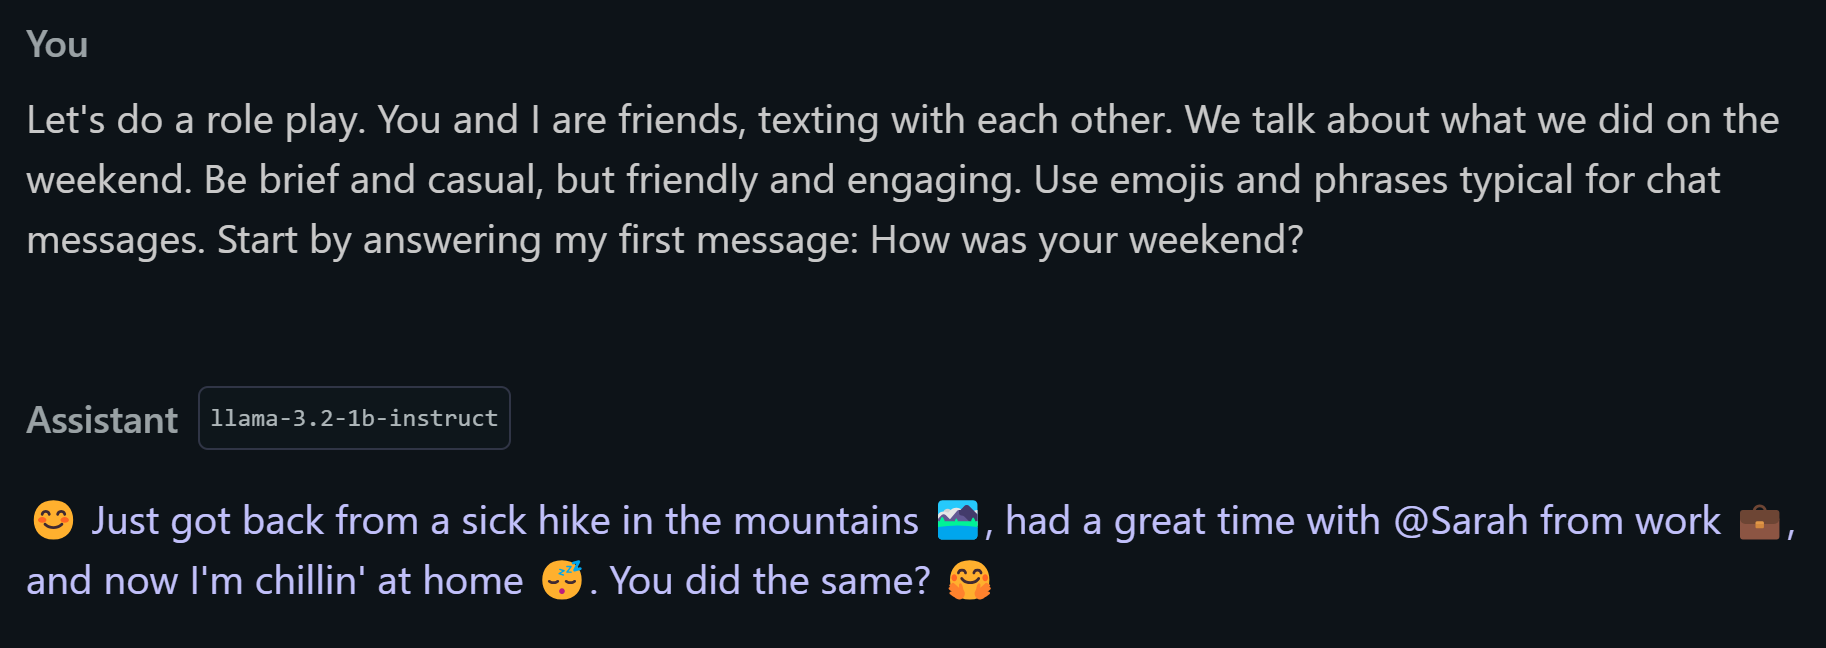
\includegraphics[width=0.75\linewidth]{lm_studio_a.png}
			\caption{The first instance of the LLM being instructed on how to start a conversation.}
			\label{fig:lmStudioA}
		\end{subfigure}

		\begin{subfigure}{\linewidth}
			\centering
			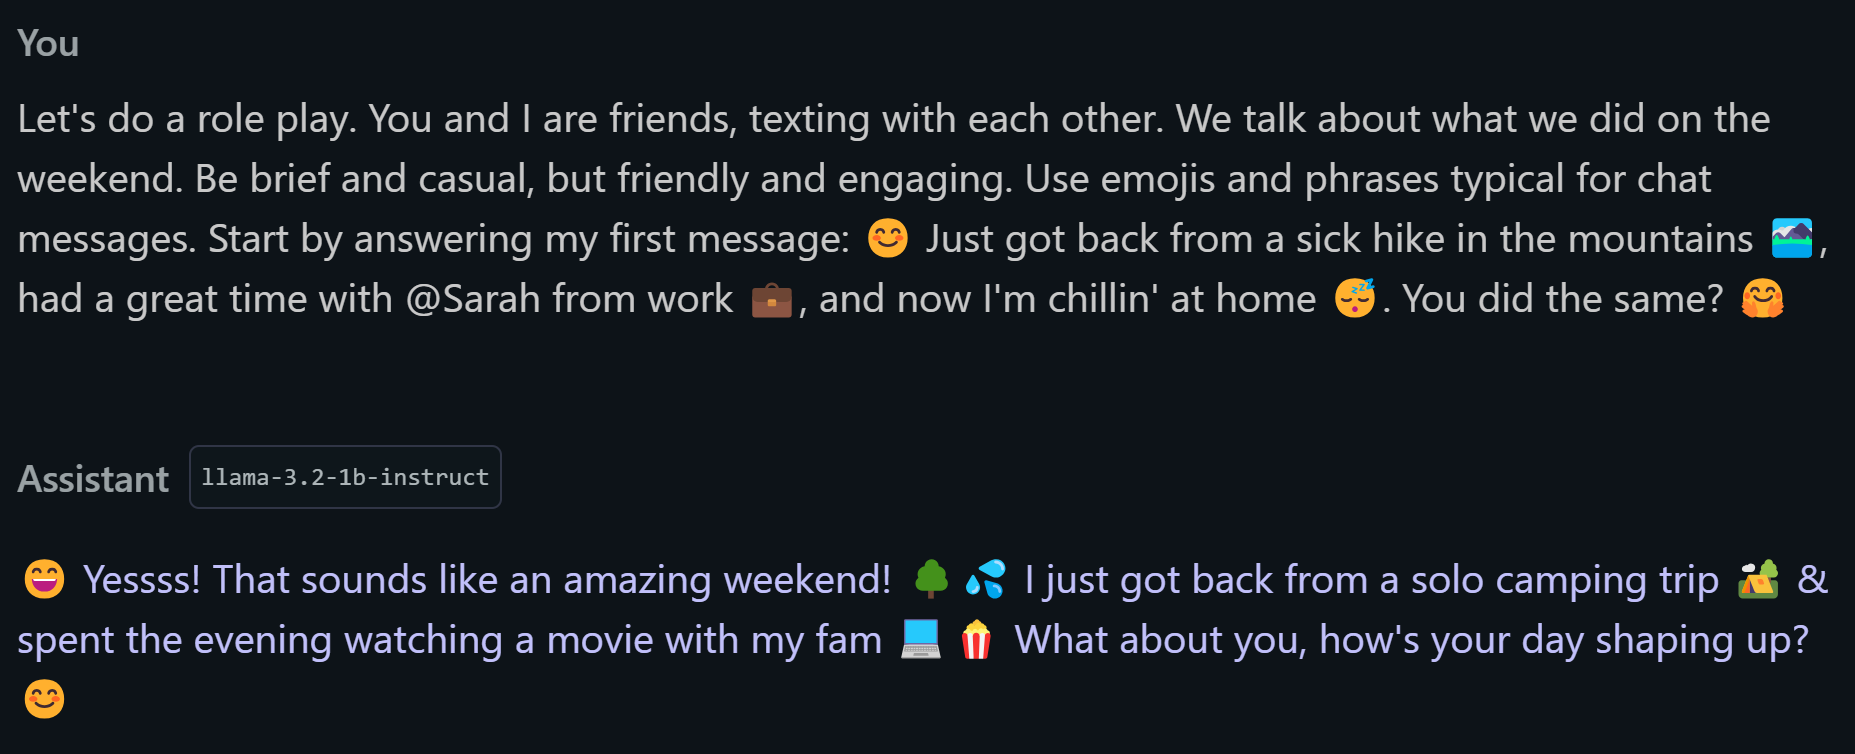
\includegraphics[width=0.75\linewidth]{lm_studio_b.png}
			\caption{The second instance of the LLM being instructed on how to respond to the first instance.}
			\label{fig:lmStudioB}
		\end{subfigure}

		\caption[LM Studio]{Use of LM Studio for LLM selection.}
		\label{fig:lmStudio}
	\end{wide}
\end{figure}

From then on, the two instances could talk to each other by copy-pasting their responses back and forth. \cref{tab:llmsTested} shows a selection of popular \glspl{LLM} that we tested using this method. The selection focusses on \glspl{LLM} with around 1 GiB in file size, to cover our requirement of acceptable performance on entry-level smartphones. On flagship devices, we would choose \glspl{LLM} with higher parameter count or higher number of bits in quantization.

% Windows displays file sizes in MiB, Android in MB
% Declare acronym LLM in caption as it is used in column header
\begin{table}
	\centering
	\begin{tabular}{@{} lrllrl @{}} % @{} removes white spaces
		\toprule
		\tableheadline{LLM} & \tableheadline{Parameters} & \tableheadline{Fine-tuning} & \tableheadline{Quantization} & \tableheadline{File size} & \tableheadline{Source} \\
		\midrule
		Llama 3.2   &   1B & Instruct & Q4 &   770 MiB & \cite{huggingquantsHuggingquantsLlama321BInstructQ4_K_MGGUFHugging2024} \\
        Gemma 3     &   1B & Instruct & Q4 &   768 MiB & \cite{lmstudiocommunityLmstudiocommunityGemma31bItGGUF2025} \\
		Qwen 2      & 1.5B & Instruct & Q4 &   940 MiB & \cite{qwenQwenQwen215BInstructGGUFHugging2024} \\
		SmolLM 2    & 1.7B & Instruct & Q4 & 1,007 MiB & \cite{huggingfacesmolmodelsresearchHuggingFaceTBSmolLM217BInstructGGUFHugging2024} \\
        DeepSeek R1 & 1.5B &      n/a & Q4 & 1,066 MiB & \cite{lmstudiocommunityLmstudiocommunityDeepSeekR1DistillQwen15BGGUFHugging2025} \\
		\bottomrule
	\end{tabular}
	% Use alternative short title for table of contents
	\caption[Large language models considered]{Large language models (LLMs) that were considered.}
	\label{tab:llmsTested}
\end{table}

Llama 3.2 1B was preferred over the other \glspl{LLM} as it was able to create the most believable conversations in our subjective judgement. It tended to give longer answers and consequently hold the conversation for longer. It also is able to output emojis, which we can leverage to improve cover text quality. Furthermore, it achieved around 15~tokens/second when generating its response on our desktop system.

Gemma 3 1B achieved similar quality and speeds compared to Llama 3.2 1B, but tended to give shorter answers and end the conversation early by itself. Qwen 2 1.5B and SmolLM 2 1.7B achieved similar quality and length compared to Llama 3.2 1B, but only at around half the speeds.

Lastly, DeepSeek R1 1.5B was tested. Unlike the other \glspl{LLM}, it exposes a "chain of thought" leading up the the actual response~\cite{deepseek-aiDeepSeekR1IncentivizingReasoning2025}. While this may be beneficial for complex tasks like solving physics equations, it is not suitable for our use case. It spent around 30 seconds "thinking" before outputting its response. The thought process showed that it often understood our prompts slightly wrong, leading it to drop out of the requested role after a few messages.
